\documentclass{whiteboard}
\begin{document}
\begin{frame}[plain,t]
\bbcover{USACO 2017 December Contest}{Silver, Problem 3: The Bovine Shuffle}{Prof. Edson Alves}{Faculdade UnB Gama}

\end{frame}
\begin{frame}[plain,t]
\vspace*{\fill}

\bbenglish{Convinced that happy cows generate more milk, Farmer John has installed a giant disco ball in his barn and plans to teach his cows to dance!}

\vspace{0.1in}

\bbenglish{Looking up popular cow dances, Farmer John decides to teach his cows the ``Bovine Shuffle''. The Bovine Shuffle consists of his $N$ cows $(1\leq N\leq 100,000)$ lining up in a row in some order, then performing successive ``shuffles'', each of which potentially re-orders the cows. To make it easier for his cows to locate themselves, Farmer John marks the locations for his line of cows with positions $1\ldots N$, so the first cow in the lineup will be in position $1$, the next in position $2$, and so on, up to position $N$.}

\vspace*{\fill}
\end{frame}
\begin{frame}[plain,t]
\vspace*{\fill}

\bbtext{Convencido que vacas felizes dão mais leite, o fazendeiro John instalou uma bola de discoteca gigante no celeiro e planeja ensinar suas vacas a dançar!}

\vspace{0.1in}

\bbtext{Procurando por danças bovinas populares, o fazendeiro John decidiu ensinar a suas vacas a ``Misturada Bovina''. A Misturada Bovina consiste em alinhar suas $N$ vacas $(1\leq N\leq 100.000)$ em uma linha, em alguma ordem. Então elas executam sucessivas ``misturas'', cada uma delas potencialmente reordenando as vacas. Para que as vacas possam se localizar com mais facilidade, o fazendeiro John marcou posições na linha com números de $1\ldots N$, de modo que a primeira vaca se alinhe na posição $1$, a próxima na posição $2$, e assim por diante, até a posição $N$.}

\vspace*{\fill}
\end{frame}
\begin{frame}[plain,t]
\vspace*{\fill}

\bbenglish{A shuffle is described with $N$ numbers, $a_1\ldots a_N$, where a cow in position $i$ moves to position $a_i$ during the shuffle (and so, each $a_i$ is in the range $1\ldots N$). Every cow moves to its new location during the shuffle. Unfortunately, all the $a_i$'s are not necessarily distinct, so multiple cows might try to move to the same position during a shuffle, after which they will move together for all remaining shuffles.}

\vspace{0.1in}

\bbenglish{Farmer John notices that some positions in his lineup contain cows in them no matter how many shuffles take place. Please help him count the number of such positions.}

\vspace*{\fill}
\end{frame}
\begin{frame}[plain,t]
\vspace*{\fill}

\bbtext{Uma mistura é descrita por $N$ números, $a_1\ldots a_N$, onde a vaca que ocupa a posição $i$ se move para a posição $a_i$ durante a mistura (e assim por diante, cada $a_i$ está no intervalo $1\ldots N$). Cada vaca se move para sua nova localização durante a mistura. Infelizmente, os $a_i$'s não são necessariamente distintos, de modo que múltiplas vacas podem tentar se mover para a mesma posição durante a mistura, e após isso elas deve se mover juntas durante todas as misturas restantes.}

\vspace{0.1in}

\bbtext{O fazendeiro John notou que algumas posições na linha sempre tinham vacas sobre elas independentemente do número de misturas feitas. Por favor o ajude a contar o número de tais posições.}

\vspace*{\fill}
\end{frame}
\begin{frame}[plain,t]
\vspace*{\fill}

\bbbold{Input}

\vspace{0.1in}

\bbenglish{The first line of input contains $N$, the number of cows. The next line contains the $N$ integers $a_1\ldots a_N$.}

\vspace{0.2in}

\bbbold{Output}

\vspace{0.1in}

\bbenglish{Please output the number of positions that will always contain cows, no matter how many shuffles take place.}

\vspace*{\fill}
\end{frame}
\begin{frame}[plain,t]
\vspace*{\fill}

\bbbold{Entrada}

\vspace{0.1in}

\bbtext{A primeira linha da entrada contém $N$, o número de vacas. A próxima linha contém os $N$ inteiros $a_1\ldots a_N$.}

\vspace{0.2in}

\bbbold{Saída}

\vspace{0.1in}

\bbtext{Por favor imprima o número de posições que sempre terão vacas, independentemente de quantas misturas sejam feitas.}

\vspace*{\fill}
\end{frame}
\begin{frame}[plain,t]
\begin{tikzpicture}
\node[draw,opacity=0] at (0, 0) {x};
\node[draw,opacity=0] at (14, 8) {x};

	\node[anchor=west] (header) at (0, 7.0) { \bbbold{Exemplo de entrada e saída} };

\end{tikzpicture}
\end{frame}
\begin{frame}[plain,t]
\begin{tikzpicture}
\node[draw,opacity=0] at (0, 0) {x};
\node[draw,opacity=0] at (14, 8) {x};

	\node[anchor=west] (header) at (0, 7.0) { \bbbold{Exemplo de entrada e saída} };


	\node[anchor=west] (line1) at (1.0, 6.0) { \bbtext{\texttt{4} } };

\end{tikzpicture}
\end{frame}
\begin{frame}[plain,t]
\begin{tikzpicture}
\node[draw,opacity=0] at (0, 0) {x};
\node[draw,opacity=0] at (14, 8) {x};

	\node[anchor=west] (header) at (0, 7.0) { \bbbold{Exemplo de entrada e saída} };


	\node[anchor=west] (line1) at (1.0, 6.0) { \bbtext{\texttt{4} } };


	\draw[->,color=BBViolet] (1.25, 5.0) to  (1.25, 5.75);

	\node[] (r) at (1.25, 4.75) { \footnotesize \bbcomment{\# de vacas} };

\end{tikzpicture}
\end{frame}
\begin{frame}[plain,t]
\begin{tikzpicture}
\node[draw,opacity=0] at (0, 0) {x};
\node[draw,opacity=0] at (14, 8) {x};

	\node[anchor=west] (header) at (0, 7.0) { \bbbold{Exemplo de entrada e saída} };


	\node[anchor=west] (line1) at (1.0, 6.0) { \bbtext{\texttt{4} } };





	\node[draw,very thick,circle] (node1) at (6.0, 4.0) { \bbtext{1} };

	\node[draw,very thick,circle] (node2) at (8.0, 4.0) { \bbtext{2} };

	\node[draw,very thick,circle] (node3) at (10.0, 4.0) { \bbtext{3} };

	\node[draw,very thick,circle] (node4) at (12.0, 4.0) { \bbtext{4} };

	\node[] (cow1) at (6.0, 5.0) { \includegraphics[scale=0.05]{figs/cow.png} };

	\node[] (cow2) at (8.0, 5.0) { \includegraphics[scale=0.05]{figs/cow.png} };

	\node[] (cow3) at (10.0, 5.0) { \includegraphics[scale=0.05]{figs/cow.png} };

	\node[] (cow4) at (12.0, 5.0) { \includegraphics[scale=0.05]{figs/cow.png} };

\end{tikzpicture}
\end{frame}
\begin{frame}[plain,t]
\begin{tikzpicture}
\node[draw,opacity=0] at (0, 0) {x};
\node[draw,opacity=0] at (14, 8) {x};

	\node[anchor=west] (header) at (0, 7.0) { \bbbold{Exemplo de entrada e saída} };


	\node[anchor=west] (line1) at (1.0, 6.0) { \bbtext{\texttt{4} } };





	\node[draw,very thick,circle] (node1) at (6.0, 4.0) { \bbtext{1} };

	\node[draw,very thick,circle] (node2) at (8.0, 4.0) { \bbtext{2} };

	\node[draw,very thick,circle] (node3) at (10.0, 4.0) { \bbtext{3} };

	\node[draw,very thick,circle] (node4) at (12.0, 4.0) { \bbtext{4} };

	\node[] (cow1) at (6.0, 5.0) { \includegraphics[scale=0.05]{figs/cow.png} };

	\node[] (cow2) at (8.0, 5.0) { \includegraphics[scale=0.05]{figs/cow.png} };

	\node[] (cow3) at (10.0, 5.0) { \includegraphics[scale=0.05]{figs/cow.png} };

	\node[] (cow4) at (12.0, 5.0) { \includegraphics[scale=0.05]{figs/cow.png} };


	\node[anchor=west] (line2) at (1.0, 5.5) { \bbtext{\texttt{3 2 1 3} } };

\end{tikzpicture}
\end{frame}
\begin{frame}[plain,t]
\begin{tikzpicture}
\node[draw,opacity=0] at (0, 0) {x};
\node[draw,opacity=0] at (14, 8) {x};

	\node[anchor=west] (header) at (0, 7.0) { \bbbold{Exemplo de entrada e saída} };


	\node[anchor=west] (line1) at (1.0, 6.0) { \bbtext{\texttt{4} } };


	\draw[->,color=BBViolet] (1.25, 4.25) to  (1.25, 5.25);

	\node[] (r) at (1.25, 4.0) { \footnotesize \bbcomment{$a_1$} };


	\node[draw,very thick,circle] (node1) at (6.0, 4.0) { \bbtext{1} };

	\node[draw,very thick,circle] (node2) at (8.0, 4.0) { \bbtext{2} };

	\node[draw,very thick,circle] (node3) at (10.0, 4.0) { \bbtext{3} };

	\node[draw,very thick,circle] (node4) at (12.0, 4.0) { \bbtext{4} };

	\node[] (cow1) at (6.0, 5.0) { \includegraphics[scale=0.05]{figs/cow.png} };

	\node[] (cow2) at (8.0, 5.0) { \includegraphics[scale=0.05]{figs/cow.png} };

	\node[] (cow3) at (10.0, 5.0) { \includegraphics[scale=0.05]{figs/cow.png} };

	\node[] (cow4) at (12.0, 5.0) { \includegraphics[scale=0.05]{figs/cow.png} };


	\node[anchor=west] (line2) at (1.0, 5.5) { \bbtext{\texttt{3 2 1 3} } };




\end{tikzpicture}
\end{frame}
\begin{frame}[plain,t]
\begin{tikzpicture}
\node[draw,opacity=0] at (0, 0) {x};
\node[draw,opacity=0] at (14, 8) {x};

	\node[anchor=west] (header) at (0, 7.0) { \bbbold{Exemplo de entrada e saída} };


	\node[anchor=west] (line1) at (1.0, 6.0) { \bbtext{\texttt{4} } };


	\draw[->,color=BBViolet] (1.25, 4.25) to  (1.25, 5.25);

	\node[] (r) at (1.25, 4.0) { \footnotesize \bbcomment{$a_1$} };


	\node[draw,very thick,circle] (node1) at (6.0, 4.0) { \bbtext{1} };

	\node[draw,very thick,circle] (node2) at (8.0, 4.0) { \bbtext{2} };

	\node[draw,very thick,circle] (node3) at (10.0, 4.0) { \bbtext{3} };

	\node[draw,very thick,circle] (node4) at (12.0, 4.0) { \bbtext{4} };

	\node[] (cow1) at (6.0, 5.0) { \includegraphics[scale=0.05]{figs/cow.png} };

	\node[] (cow2) at (8.0, 5.0) { \includegraphics[scale=0.05]{figs/cow.png} };

	\node[] (cow3) at (10.0, 5.0) { \includegraphics[scale=0.05]{figs/cow.png} };

	\node[] (cow4) at (12.0, 5.0) { \includegraphics[scale=0.05]{figs/cow.png} };


	\node[anchor=west] (line2) at (1.0, 5.5) { \bbtext{\texttt{3 2 1 3} } };





	\draw[thick,-latex](node1) to [bend right] (node3);

\end{tikzpicture}
\end{frame}
\begin{frame}[plain,t]
\begin{tikzpicture}
\node[draw,opacity=0] at (0, 0) {x};
\node[draw,opacity=0] at (14, 8) {x};

	\node[anchor=west] (header) at (0, 7.0) { \bbbold{Exemplo de entrada e saída} };


	\node[anchor=west] (line1) at (1.0, 6.0) { \bbtext{\texttt{4} } };


	\draw[->,color=BBViolet] (1.65, 4.25) to  (1.65, 5.25);

	\node[] (r) at (1.65, 4.0) { \footnotesize \bbcomment{$a_2$} };


	\node[draw,very thick,circle] (node1) at (6.0, 4.0) { \bbtext{1} };

	\node[draw,very thick,circle] (node2) at (8.0, 4.0) { \bbtext{2} };

	\node[draw,very thick,circle] (node3) at (10.0, 4.0) { \bbtext{3} };

	\node[draw,very thick,circle] (node4) at (12.0, 4.0) { \bbtext{4} };

	\node[] (cow1) at (6.0, 5.0) { \includegraphics[scale=0.05]{figs/cow.png} };

	\node[] (cow2) at (8.0, 5.0) { \includegraphics[scale=0.05]{figs/cow.png} };

	\node[] (cow3) at (10.0, 5.0) { \includegraphics[scale=0.05]{figs/cow.png} };

	\node[] (cow4) at (12.0, 5.0) { \includegraphics[scale=0.05]{figs/cow.png} };


	\node[anchor=west] (line2) at (1.0, 5.5) { \bbtext{\texttt{3 2 1 3} } };





	\draw[thick,-latex](node1) to [bend right] (node3);




\end{tikzpicture}
\end{frame}
\begin{frame}[plain,t]
\begin{tikzpicture}
\node[draw,opacity=0] at (0, 0) {x};
\node[draw,opacity=0] at (14, 8) {x};

	\node[anchor=west] (header) at (0, 7.0) { \bbbold{Exemplo de entrada e saída} };


	\node[anchor=west] (line1) at (1.0, 6.0) { \bbtext{\texttt{4} } };


	\draw[->,color=BBViolet] (1.65, 4.25) to  (1.65, 5.25);

	\node[] (r) at (1.65, 4.0) { \footnotesize \bbcomment{$a_2$} };


	\node[draw,very thick,circle] (node1) at (6.0, 4.0) { \bbtext{1} };

	\node[draw,very thick,circle] (node2) at (8.0, 4.0) { \bbtext{2} };

	\node[draw,very thick,circle] (node3) at (10.0, 4.0) { \bbtext{3} };

	\node[draw,very thick,circle] (node4) at (12.0, 4.0) { \bbtext{4} };

	\node[] (cow1) at (6.0, 5.0) { \includegraphics[scale=0.05]{figs/cow.png} };

	\node[] (cow2) at (8.0, 5.0) { \includegraphics[scale=0.05]{figs/cow.png} };

	\node[] (cow3) at (10.0, 5.0) { \includegraphics[scale=0.05]{figs/cow.png} };

	\node[] (cow4) at (12.0, 5.0) { \includegraphics[scale=0.05]{figs/cow.png} };


	\node[anchor=west] (line2) at (1.0, 5.5) { \bbtext{\texttt{3 2 1 3} } };





	\draw[thick,-latex](node1) to [bend right] (node3);





	\draw[thick,-latex](node2) to [loop left] (node2);


\end{tikzpicture}
\end{frame}
\begin{frame}[plain,t]
\begin{tikzpicture}
\node[draw,opacity=0] at (0, 0) {x};
\node[draw,opacity=0] at (14, 8) {x};

	\node[anchor=west] (header) at (0, 7.0) { \bbbold{Exemplo de entrada e saída} };


	\node[anchor=west] (line1) at (1.0, 6.0) { \bbtext{\texttt{4} } };


	\draw[->,color=BBViolet] (2.05, 4.25) to  (2.05, 5.25);

	\node[] (r) at (2.05, 4.0) { \footnotesize \bbcomment{$a_3$} };


	\node[draw,very thick,circle] (node1) at (6.0, 4.0) { \bbtext{1} };

	\node[draw,very thick,circle] (node2) at (8.0, 4.0) { \bbtext{2} };

	\node[draw,very thick,circle] (node3) at (10.0, 4.0) { \bbtext{3} };

	\node[draw,very thick,circle] (node4) at (12.0, 4.0) { \bbtext{4} };

	\node[] (cow1) at (6.0, 5.0) { \includegraphics[scale=0.05]{figs/cow.png} };

	\node[] (cow2) at (8.0, 5.0) { \includegraphics[scale=0.05]{figs/cow.png} };

	\node[] (cow3) at (10.0, 5.0) { \includegraphics[scale=0.05]{figs/cow.png} };

	\node[] (cow4) at (12.0, 5.0) { \includegraphics[scale=0.05]{figs/cow.png} };


	\node[anchor=west] (line2) at (1.0, 5.5) { \bbtext{\texttt{3 2 1 3} } };





	\draw[thick,-latex](node1) to [bend right] (node3);





	\draw[thick,-latex](node2) to [loop left] (node2);




\end{tikzpicture}
\end{frame}
\begin{frame}[plain,t]
\begin{tikzpicture}
\node[draw,opacity=0] at (0, 0) {x};
\node[draw,opacity=0] at (14, 8) {x};

	\node[anchor=west] (header) at (0, 7.0) { \bbbold{Exemplo de entrada e saída} };


	\node[anchor=west] (line1) at (1.0, 6.0) { \bbtext{\texttt{4} } };


	\draw[->,color=BBViolet] (2.05, 4.25) to  (2.05, 5.25);

	\node[] (r) at (2.05, 4.0) { \footnotesize \bbcomment{$a_3$} };


	\node[draw,very thick,circle] (node1) at (6.0, 4.0) { \bbtext{1} };

	\node[draw,very thick,circle] (node2) at (8.0, 4.0) { \bbtext{2} };

	\node[draw,very thick,circle] (node3) at (10.0, 4.0) { \bbtext{3} };

	\node[draw,very thick,circle] (node4) at (12.0, 4.0) { \bbtext{4} };

	\node[] (cow1) at (6.0, 5.0) { \includegraphics[scale=0.05]{figs/cow.png} };

	\node[] (cow2) at (8.0, 5.0) { \includegraphics[scale=0.05]{figs/cow.png} };

	\node[] (cow3) at (10.0, 5.0) { \includegraphics[scale=0.05]{figs/cow.png} };

	\node[] (cow4) at (12.0, 5.0) { \includegraphics[scale=0.05]{figs/cow.png} };


	\node[anchor=west] (line2) at (1.0, 5.5) { \bbtext{\texttt{3 2 1 3} } };





	\draw[thick,-latex,latex-latex](node1) to [bend right] (node3);





	\draw[thick,-latex](node2) to [loop left] (node2);





\end{tikzpicture}
\end{frame}
\begin{frame}[plain,t]
\begin{tikzpicture}
\node[draw,opacity=0] at (0, 0) {x};
\node[draw,opacity=0] at (14, 8) {x};

	\node[anchor=west] (header) at (0, 7.0) { \bbbold{Exemplo de entrada e saída} };


	\node[anchor=west] (line1) at (1.0, 6.0) { \bbtext{\texttt{4} } };


	\draw[->,color=BBViolet] (2.45, 4.25) to  (2.45, 5.25);

	\node[] (r) at (2.45, 4.0) { \footnotesize \bbcomment{$a_4$} };


	\node[draw,very thick,circle] (node1) at (6.0, 4.0) { \bbtext{1} };

	\node[draw,very thick,circle] (node2) at (8.0, 4.0) { \bbtext{2} };

	\node[draw,very thick,circle] (node3) at (10.0, 4.0) { \bbtext{3} };

	\node[draw,very thick,circle] (node4) at (12.0, 4.0) { \bbtext{4} };

	\node[] (cow1) at (6.0, 5.0) { \includegraphics[scale=0.05]{figs/cow.png} };

	\node[] (cow2) at (8.0, 5.0) { \includegraphics[scale=0.05]{figs/cow.png} };

	\node[] (cow3) at (10.0, 5.0) { \includegraphics[scale=0.05]{figs/cow.png} };

	\node[] (cow4) at (12.0, 5.0) { \includegraphics[scale=0.05]{figs/cow.png} };


	\node[anchor=west] (line2) at (1.0, 5.5) { \bbtext{\texttt{3 2 1 3} } };





	\draw[thick,-latex,latex-latex](node1) to [bend right] (node3);





	\draw[thick,-latex](node2) to [loop left] (node2);







\end{tikzpicture}
\end{frame}
\begin{frame}[plain,t]
\begin{tikzpicture}
\node[draw,opacity=0] at (0, 0) {x};
\node[draw,opacity=0] at (14, 8) {x};

	\node[anchor=west] (header) at (0, 7.0) { \bbbold{Exemplo de entrada e saída} };


	\node[anchor=west] (line1) at (1.0, 6.0) { \bbtext{\texttt{4} } };


	\draw[->,color=BBViolet] (2.45, 4.25) to  (2.45, 5.25);

	\node[] (r) at (2.45, 4.0) { \footnotesize \bbcomment{$a_4$} };


	\node[draw,very thick,circle] (node1) at (6.0, 4.0) { \bbtext{1} };

	\node[draw,very thick,circle] (node2) at (8.0, 4.0) { \bbtext{2} };

	\node[draw,very thick,circle] (node3) at (10.0, 4.0) { \bbtext{3} };

	\node[draw,very thick,circle] (node4) at (12.0, 4.0) { \bbtext{4} };

	\node[] (cow1) at (6.0, 5.0) { \includegraphics[scale=0.05]{figs/cow.png} };

	\node[] (cow2) at (8.0, 5.0) { \includegraphics[scale=0.05]{figs/cow.png} };

	\node[] (cow3) at (10.0, 5.0) { \includegraphics[scale=0.05]{figs/cow.png} };

	\node[] (cow4) at (12.0, 5.0) { \includegraphics[scale=0.05]{figs/cow.png} };


	\node[anchor=west] (line2) at (1.0, 5.5) { \bbtext{\texttt{3 2 1 3} } };





	\draw[thick,-latex,latex-latex](node1) to [bend right] (node3);





	\draw[thick,-latex](node2) to [loop left] (node2);








	\draw[thick,-latex](node4) to (node3);

\end{tikzpicture}
\end{frame}
\begin{frame}[plain,t]
\begin{tikzpicture}
\node[draw,opacity=0] at (0, 0) {x};
\node[draw,opacity=0] at (14, 8) {x};

	\node[anchor=west] (header) at (0, 7.0) { \bbbold{Exemplo de entrada e saída} };


	\node[anchor=west] (line1) at (1.0, 6.0) { \bbtext{\texttt{4} } };





	\node[draw,very thick,circle] (node1) at (6.0, 4.0) { \bbtext{1} };

	\node[draw,very thick,circle] (node2) at (8.0, 4.0) { \bbtext{2} };

	\node[draw,very thick,circle] (node3) at (10.0, 4.0) { \bbtext{3} };

	\node[draw,very thick,circle] (node4) at (12.0, 4.0) { \bbtext{4} };

	\node[] (cow1) at (6.0, 5.0) { \includegraphics[scale=0.05]{figs/cow.png} };

	\node[] (cow2) at (8.0, 5.0) { \includegraphics[scale=0.05]{figs/cow.png} };

	\node[] (cow3) at (10.0, 5.0) { \includegraphics[scale=0.05]{figs/cow.png} };

	\node[] (cow4) at (12.0, 5.0) { \includegraphics[scale=0.05]{figs/cow.png} };


	\node[anchor=west] (line2) at (1.0, 5.5) { \bbtext{\texttt{3 2 1 3} } };





	\draw[thick,-latex,latex-latex](node1) to [bend right] (node3);





	\draw[thick,-latex](node2) to [loop left] (node2);








	\draw[thick,-latex](node4) to (node3);


\end{tikzpicture}
\end{frame}
\begin{frame}[plain,t]
\begin{tikzpicture}
\node[draw,opacity=0] at (0, 0) {x};
\node[draw,opacity=0] at (14, 8) {x};

	\node[anchor=west] (header) at (0, 7.0) { \bbbold{Exemplo de entrada e saída} };


	\node[anchor=west] (line1) at (1.0, 6.0) { \bbtext{\texttt{4} } };





	\node[draw,very thick,circle] (node1) at (6.0, 4.0) { \bbtext{1} };

	\node[draw,very thick,circle] (node2) at (8.0, 4.0) { \bbtext{2} };

	\node[draw,very thick,circle] (node3) at (10.0, 4.0) { \bbtext{3} };

	\node[draw,very thick,circle] (node4) at (12.0, 4.0) { \bbtext{4} };

	\node[] (cow1) at (6.0, 5.0) { \includegraphics[scale=0.05]{figs/cow.png} };

	\node[] (cow2) at (8.0, 5.0) { \includegraphics[scale=0.05]{figs/cow.png} };

	\node[] (cow3) at (10.0, 5.0) { \includegraphics[scale=0.05]{figs/cow.png} };

	\node[] (cow4) at (12.0, 5.0) { \includegraphics[scale=0.05]{figs/cow.png} };


	\node[anchor=west] (line2) at (1.0, 5.5) { \bbtext{\texttt{3 2 1 3} } };





	\draw[thick,-latex,latex-latex](node1) to [bend right] (node3);





	\draw[thick,-latex](node2) to [loop left] (node2);








	\draw[thick,-latex](node4) to (node3);



	\node[] (info) at (9.0, 2.0) { \bbbold{Mistura \#1} };

\end{tikzpicture}
\end{frame}
\begin{frame}[plain,t]
\begin{tikzpicture}
\node[draw,opacity=0] at (0, 0) {x};
\node[draw,opacity=0] at (14, 8) {x};

	\node[anchor=west] (header) at (0, 7.0) { \bbbold{Exemplo de entrada e saída} };


	\node[anchor=west] (line1) at (1.0, 6.0) { \bbtext{\texttt{4} } };





	\node[draw,very thick,circle] (node1) at (6.0, 4.0) { \bbtext{1} };

	\node[draw,very thick,circle] (node2) at (8.0, 4.0) { \bbtext{2} };

	\node[draw,very thick,circle] (node3) at (10.0, 4.0) { \bbtext{3} };

	\node[draw,very thick,circle] (node4) at (12.0, 4.0) { \bbtext{4} };

	\node[] (cow1) at (6.0, 5.0) { \includegraphics[scale=0.05]{figs/cow.png} };

	\node[] (cow2) at (8.0, 5.0) { \includegraphics[scale=0.05]{figs/cow.png} };

	\node[] (cow3) at (10.0, 5.0) { \includegraphics[scale=0.05]{figs/cow.png} };

	\node[] (cow4) at (10.0, 5.75) { \includegraphics[scale=0.05]{figs/cow.png} };


	\node[anchor=west] (line2) at (1.0, 5.5) { \bbtext{\texttt{3 2 1 3} } };





	\draw[thick,-latex,latex-latex](node1) to [bend right] (node3);





	\draw[thick,-latex](node2) to [loop left] (node2);








	\draw[thick,-latex](node4) to (node3);



	\node[] (info) at (9.0, 2.0) { \bbbold{Mistura \#1} };


\end{tikzpicture}
\end{frame}
\begin{frame}[plain,t]
\begin{tikzpicture}
\node[draw,opacity=0] at (0, 0) {x};
\node[draw,opacity=0] at (14, 8) {x};

	\node[anchor=west] (header) at (0, 7.0) { \bbbold{Exemplo de entrada e saída} };


	\node[anchor=west] (line1) at (1.0, 6.0) { \bbtext{\texttt{4} } };





	\node[draw,very thick,circle] (node1) at (6.0, 4.0) { \bbtext{1} };

	\node[draw,very thick,circle] (node2) at (8.0, 4.0) { \bbtext{2} };

	\node[draw,very thick,circle] (node3) at (10.0, 4.0) { \bbtext{3} };

	\node[draw,very thick,circle] (node4) at (12.0, 4.0) { \bbtext{4} };

	\node[] (cow1) at (6.0, 5.0) { \includegraphics[scale=0.05]{figs/cow.png} };

	\node[] (cow2) at (8.0, 5.0) { \includegraphics[scale=0.05]{figs/cow.png} };

	\node[] (cow3) at (10.0, 5.0) { \includegraphics[scale=0.05]{figs/cow.png} };

	\node[] (cow4) at (10.0, 5.75) { \includegraphics[scale=0.05]{figs/cow.png} };


	\node[anchor=west] (line2) at (1.0, 5.5) { \bbtext{\texttt{3 2 1 3} } };





	\draw[thick,-latex,latex-latex](node1) to [bend right] (node3);





	\draw[thick,-latex](node2) to [loop left] (node2);








	\draw[thick,-latex](node4) to (node3);



	\node[] (info) at (9.0, 2.0) { \bbbold{Mistura \#2} };


\end{tikzpicture}
\end{frame}
\begin{frame}[plain,t]
\begin{tikzpicture}
\node[draw,opacity=0] at (0, 0) {x};
\node[draw,opacity=0] at (14, 8) {x};

	\node[anchor=west] (header) at (0, 7.0) { \bbbold{Exemplo de entrada e saída} };


	\node[anchor=west] (line1) at (1.0, 6.0) { \bbtext{\texttt{4} } };





	\node[draw,very thick,circle] (node1) at (6.0, 4.0) { \bbtext{1} };

	\node[draw,very thick,circle] (node2) at (8.0, 4.0) { \bbtext{2} };

	\node[draw,very thick,circle] (node3) at (10.0, 4.0) { \bbtext{3} };

	\node[draw,very thick,circle] (node4) at (12.0, 4.0) { \bbtext{4} };

	\node[] (cow1) at (6.0, 5.0) { \includegraphics[scale=0.05]{figs/cow.png} };

	\node[] (cow2) at (8.0, 5.0) { \includegraphics[scale=0.05]{figs/cow.png} };

	\node[] (cow3) at (10.0, 5.0) { \includegraphics[scale=0.05]{figs/cow.png} };

	\node[] (cow4) at (6.0, 5.75) { \includegraphics[scale=0.05]{figs/cow.png} };


	\node[anchor=west] (line2) at (1.0, 5.5) { \bbtext{\texttt{3 2 1 3} } };





	\draw[thick,-latex,latex-latex](node1) to [bend right] (node3);





	\draw[thick,-latex](node2) to [loop left] (node2);








	\draw[thick,-latex](node4) to (node3);



	\node[] (info) at (9.0, 2.0) { \bbbold{Mistura \#2} };



\end{tikzpicture}
\end{frame}
\begin{frame}[plain,t]
\begin{tikzpicture}
\node[draw,opacity=0] at (0, 0) {x};
\node[draw,opacity=0] at (14, 8) {x};

	\node[anchor=west] (header) at (0, 7.0) { \bbbold{Exemplo de entrada e saída} };


	\node[anchor=west] (line1) at (1.0, 6.0) { \bbtext{\texttt{4} } };


	\draw[->,color=BBBlack,very thick,-latex] (1.85, 5.25) to  (1.85, 4.25);

	\node[] (r) at (1.85, 4.0) { \footnotesize \bboutput{3} };


	\node[draw,very thick,circle] (node1) at (6.0, 4.0) { \bbtext{1} };

	\node[draw,very thick,circle] (node2) at (8.0, 4.0) { \bbtext{2} };

	\node[draw,very thick,circle] (node3) at (10.0, 4.0) { \bbtext{3} };

	\node[draw,very thick,circle] (node4) at (12.0, 4.0) { \bbtext{4} };

	\node[] (cow1) at (6.0, 5.0) { \includegraphics[scale=0.05]{figs/cow.png} };

	\node[] (cow2) at (8.0, 5.0) { \includegraphics[scale=0.05]{figs/cow.png} };

	\node[] (cow3) at (10.0, 5.0) { \includegraphics[scale=0.05]{figs/cow.png} };

	\node[] (cow4) at (6.0, 5.75) { \includegraphics[scale=0.05]{figs/cow.png} };


	\node[anchor=west] (line2) at (1.0, 5.5) { \bbtext{\texttt{3 2 1 3} } };





	\draw[thick,-latex,latex-latex](node1) to [bend right] (node3);





	\draw[thick,-latex](node2) to [loop left] (node2);








	\draw[thick,-latex](node4) to (node3);



	\node[] (info) at (9.0, 2.0) { \bbbold{Mistura \#2} };






\end{tikzpicture}
\end{frame}
\begin{frame}[plain,t]
\begin{tikzpicture}
\node[draw,opacity=0] at (0, 0) {x};
\node[draw,opacity=0] at (14, 8) {x};

	\node[anchor=west] (title) at (0.0, 7.0) { \Large \bbbold{Solução} };
\end{tikzpicture}
\end{frame}
\begin{frame}[plain,t]
\begin{tikzpicture}
\node[draw,opacity=0] at (0, 0) {x};
\node[draw,opacity=0] at (14, 8) {x};

	\node[anchor=west] (title) at (0.0, 7.0) { \Large \bbbold{Solução} };

	\node[] (a) at (7.0, 6.0) { \bbtext{No problema, as posições são os vértices e as movimentações as arestas} };

	\node[] (b) at (7.0, 5.25) { \bbtext{de um grafo $G$} };

\end{tikzpicture}
\end{frame}
\begin{frame}[plain,t]
\begin{tikzpicture}
\node[draw,opacity=0] at (0, 0) {x};
\node[draw,opacity=0] at (14, 8) {x};

	\node[anchor=west] (title) at (0.0, 7.0) { \Large \bbbold{Solução} };

	\node[] (a) at (7.0, 6.0) { \bbtext{Este grafo $G$ é um grafo de sucessores} };



\end{tikzpicture}
\end{frame}
\begin{frame}[plain,t]
\begin{tikzpicture}
\node[draw,opacity=0] at (0, 0) {x};
\node[draw,opacity=0] at (14, 8) {x};

	\node[anchor=west] (title) at (0.0, 7.0) { \Large \bbbold{Solução} };

	\node[] (a) at (7.0, 6.0) { \bbtext{Assim, ele tem um mais um componentes, onde cada componente tem um ciclo} };

	\node[] (b) at (7.0, 5.25) { \bbtext{e um ou mais caminhos que levam a este ciclo} };



\end{tikzpicture}
\end{frame}
\begin{frame}[plain,t]
\begin{tikzpicture}
\node[draw,opacity=0] at (0, 0) {x};
\node[draw,opacity=0] at (14, 8) {x};

	\node[anchor=west] (title) at (0.0, 7.0) { \Large \bbbold{Solução} };

	\node[] (a) at (7.0, 6.0) { \bbtext{Assim, ele tem um mais um componentes, onde cada componente tem um ciclo} };

	\node[] (b) at (7.0, 5.25) { \bbtext{e um ou mais caminhos que levam a este ciclo} };




	\node[draw,circle,thick] (a1) at (0.8, 2.0) {  };

	\node[draw,circle,thick] (a2) at (2.4, 4.0) {  };

	\node[draw,circle,thick] (a3) at (4.0, 2.0) {  };

	\node[draw,circle,thick] (a4) at (3.2, 0.0) {  };

	\node[draw,circle,thick] (a5) at (1.6, 0.0) {  };

	\draw[-latex,thick](a1) to (a2);

	\draw[-latex,thick](a2) to (a3);

	\draw[-latex,thick](a3) to (a4);

	\draw[-latex,thick](a4) to (a5);

	\draw[-latex,thick](a5) to (a1);

\end{tikzpicture}
\end{frame}
\begin{frame}[plain,t]
\begin{tikzpicture}
\node[draw,opacity=0] at (0, 0) {x};
\node[draw,opacity=0] at (14, 8) {x};

	\node[anchor=west] (title) at (0.0, 7.0) { \Large \bbbold{Solução} };

	\node[] (a) at (7.0, 6.0) { \bbtext{Assim, ele tem um mais um componentes, onde cada componente tem um ciclo} };

	\node[] (b) at (7.0, 5.25) { \bbtext{e um ou mais caminhos que levam a este ciclo} };




	\node[draw,circle,thick] (a1) at (0.8, 2.0) {  };

	\node[draw,circle,thick] (a2) at (2.4, 4.0) {  };

	\node[draw,circle,thick] (a3) at (4.0, 2.0) {  };

	\node[draw,circle,thick] (a4) at (3.2, 0.0) {  };

	\node[draw,circle,thick] (a5) at (1.6, 0.0) {  };

	\draw[-latex,thick](a1) to (a2);

	\draw[-latex,thick](a2) to (a3);

	\draw[-latex,thick](a3) to (a4);

	\draw[-latex,thick](a4) to (a5);

	\draw[-latex,thick](a5) to (a1);


	\node[draw,circle,thick] (b1) at (5.5, 3.0) {  };

	\node[draw,circle,thick] (b2) at (6.5, 3.0) {  };

	\node[draw,circle,thick] (b3) at (7.5, 3.0) {  };

	\node[draw,circle,thick] (b4) at (8.5, 3.0) {  };

	\draw[-latex,thick](b1) to (b2);

	\draw[-latex,thick](b2) to (b3);

	\draw[-latex,thick](b3) to (b4);

	\draw[-latex,thick](b4) to [bend right] (b3);

\end{tikzpicture}
\end{frame}
\begin{frame}[plain,t]
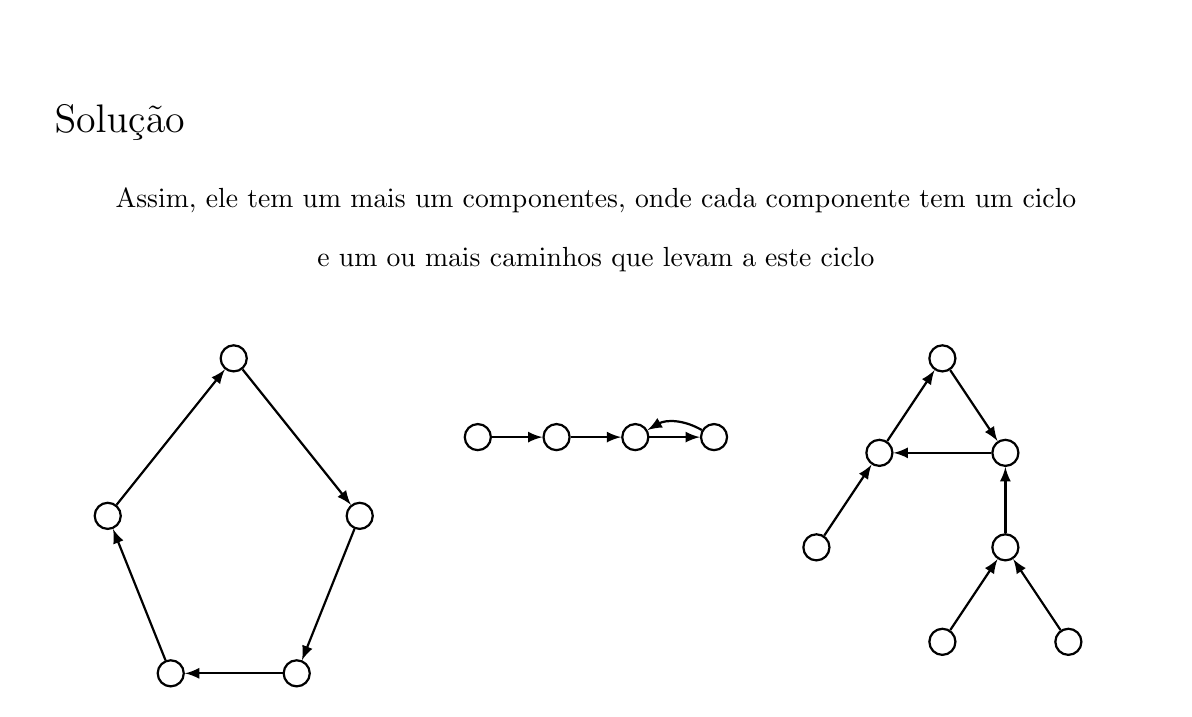
\begin{tikzpicture}
\node[draw,opacity=0] at (0, 0) {x};
\node[draw,opacity=0] at (14, 8) {x};

	\node[anchor=west] (title) at (0.0, 7.0) { \Large \bbbold{Solução} };

	\node[] (a) at (7.0, 6.0) { \bbtext{Assim, ele tem um mais um componentes, onde cada componente tem um ciclo} };

	\node[] (b) at (7.0, 5.25) { \bbtext{e um ou mais caminhos que levam a este ciclo} };




	\node[draw,circle,thick] (a1) at (0.8, 2.0) {  };

	\node[draw,circle,thick] (a2) at (2.4, 4.0) {  };

	\node[draw,circle,thick] (a3) at (4.0, 2.0) {  };

	\node[draw,circle,thick] (a4) at (3.2, 0.0) {  };

	\node[draw,circle,thick] (a5) at (1.6, 0.0) {  };

	\draw[-latex,thick](a1) to (a2);

	\draw[-latex,thick](a2) to (a3);

	\draw[-latex,thick](a3) to (a4);

	\draw[-latex,thick](a4) to (a5);

	\draw[-latex,thick](a5) to (a1);


	\node[draw,circle,thick] (b1) at (5.5, 3.0) {  };

	\node[draw,circle,thick] (b2) at (6.5, 3.0) {  };

	\node[draw,circle,thick] (b3) at (7.5, 3.0) {  };

	\node[draw,circle,thick] (b4) at (8.5, 3.0) {  };

	\draw[-latex,thick](b1) to (b2);

	\draw[-latex,thick](b2) to (b3);

	\draw[-latex,thick](b3) to (b4);

	\draw[-latex,thick](b4) to [bend right] (b3);


	\node[draw,circle,thick] (c1) at (9.8, 1.6) {  };

	\node[draw,circle,thick] (c2) at (10.6, 2.8) {  };

	\node[draw,circle,thick] (c3) at (11.4, 4.0) {  };

	\node[draw,circle,thick] (c4) at (12.2, 2.8) {  };

	\node[draw,circle,thick] (c5) at (12.2, 1.6) {  };

	\node[draw,circle,thick] (c6) at (11.4, 0.4) {  };

	\node[draw,circle,thick] (c7) at (13.0, 0.4) {  };

	\draw[-latex,thick](c1) to (c2);

	\draw[-latex,thick](c2) to (c3);

	\draw[-latex,thick](c3) to (c4);

	\draw[-latex,thick](c4) to (c2);

	\draw[-latex,thick](c5) to (c4);

	\draw[-latex,thick](c6) to (c5);

	\draw[-latex,thick](c7) to (c5);

\end{tikzpicture}
\end{frame}
\begin{frame}[plain,t]
\begin{tikzpicture}
\node[draw,opacity=0] at (0, 0) {x};
\node[draw,opacity=0] at (14, 8) {x};

	\node[anchor=west] (title) at (0.0, 7.0) { \Large \bbbold{Solução} };

	\node[] (a) at (7.0, 6.0) { \bbtext{As vacas convergem, a cada mistura, para os ciclos} };





	\node[draw,circle,thick] (a1) at (0.8, 2.0) {  };

	\node[draw,circle,thick] (a2) at (2.4, 4.0) {  };

	\node[draw,circle,thick] (a3) at (4.0, 2.0) {  };

	\node[draw,circle,thick] (a4) at (3.2, 0.0) {  };

	\node[draw,circle,thick] (a5) at (1.6, 0.0) {  };

	\draw[-latex,thick](a1) to (a2);

	\draw[-latex,thick](a2) to (a3);

	\draw[-latex,thick](a3) to (a4);

	\draw[-latex,thick](a4) to (a5);

	\draw[-latex,thick](a5) to (a1);


	\node[draw,circle,thick] (b1) at (5.5, 3.0) {  };

	\node[draw,circle,thick] (b2) at (6.5, 3.0) {  };

	\node[draw,circle,thick] (b3) at (7.5, 3.0) {  };

	\node[draw,circle,thick] (b4) at (8.5, 3.0) {  };

	\draw[-latex,thick](b1) to (b2);

	\draw[-latex,thick](b2) to (b3);

	\draw[-latex,thick](b3) to (b4);

	\draw[-latex,thick](b4) to [bend right] (b3);


	\node[draw,circle,thick] (c1) at (9.8, 1.6) {  };

	\node[draw,circle,thick] (c2) at (10.6, 2.8) {  };

	\node[draw,circle,thick] (c3) at (11.4, 4.0) {  };

	\node[draw,circle,thick] (c4) at (12.2, 2.8) {  };

	\node[draw,circle,thick] (c5) at (12.2, 1.6) {  };

	\node[draw,circle,thick] (c6) at (11.4, 0.4) {  };

	\node[draw,circle,thick] (c7) at (13.0, 0.4) {  };

	\draw[-latex,thick](c1) to (c2);

	\draw[-latex,thick](c2) to (c3);

	\draw[-latex,thick](c3) to (c4);

	\draw[-latex,thick](c4) to (c2);

	\draw[-latex,thick](c5) to (c4);

	\draw[-latex,thick](c6) to (c5);

	\draw[-latex,thick](c7) to (c5);


\end{tikzpicture}
\end{frame}
\begin{frame}[plain,t]
\begin{tikzpicture}
\node[draw,opacity=0] at (0, 0) {x};
\node[draw,opacity=0] at (14, 8) {x};

	\node[anchor=west] (title) at (0.0, 7.0) { \Large \bbbold{Solução} };

	\node[] (a) at (7.0, 6.0) { \bbtext{As vacas convergem, a cada mistura, para os ciclos} };





	\node[draw,circle,thick,fill=BBCyan] (a1) at (0.8, 2.0) {  };

	\node[draw,circle,thick,fill=BBCyan] (a2) at (2.4, 4.0) {  };

	\node[draw,circle,thick,fill=BBCyan] (a3) at (4.0, 2.0) {  };

	\node[draw,circle,thick,fill=BBCyan] (a4) at (3.2, 0.0) {  };

	\node[draw,circle,thick,fill=BBCyan] (a5) at (1.6, 0.0) {  };

	\draw[-latex,thick](a1) to (a2);

	\draw[-latex,thick](a2) to (a3);

	\draw[-latex,thick](a3) to (a4);

	\draw[-latex,thick](a4) to (a5);

	\draw[-latex,thick](a5) to (a1);


	\node[draw,circle,thick] (b1) at (5.5, 3.0) {  };

	\node[draw,circle,thick] (b2) at (6.5, 3.0) {  };

	\node[draw,circle,thick] (b3) at (7.5, 3.0) {  };

	\node[draw,circle,thick] (b4) at (8.5, 3.0) {  };

	\draw[-latex,thick](b1) to (b2);

	\draw[-latex,thick](b2) to (b3);

	\draw[-latex,thick](b3) to (b4);

	\draw[-latex,thick](b4) to [bend right] (b3);


	\node[draw,circle,thick] (c1) at (9.8, 1.6) {  };

	\node[draw,circle,thick] (c2) at (10.6, 2.8) {  };

	\node[draw,circle,thick] (c3) at (11.4, 4.0) {  };

	\node[draw,circle,thick] (c4) at (12.2, 2.8) {  };

	\node[draw,circle,thick] (c5) at (12.2, 1.6) {  };

	\node[draw,circle,thick] (c6) at (11.4, 0.4) {  };

	\node[draw,circle,thick] (c7) at (13.0, 0.4) {  };

	\draw[-latex,thick](c1) to (c2);

	\draw[-latex,thick](c2) to (c3);

	\draw[-latex,thick](c3) to (c4);

	\draw[-latex,thick](c4) to (c2);

	\draw[-latex,thick](c5) to (c4);

	\draw[-latex,thick](c6) to (c5);

	\draw[-latex,thick](c7) to (c5);



\end{tikzpicture}
\end{frame}
\begin{frame}[plain,t]
\begin{tikzpicture}
\node[draw,opacity=0] at (0, 0) {x};
\node[draw,opacity=0] at (14, 8) {x};

	\node[anchor=west] (title) at (0.0, 7.0) { \Large \bbbold{Solução} };

	\node[] (a) at (7.0, 6.0) { \bbtext{As vacas convergem, a cada mistura, para os ciclos} };





	\node[draw,circle,thick,fill=BBCyan] (a1) at (0.8, 2.0) {  };

	\node[draw,circle,thick,fill=BBCyan] (a2) at (2.4, 4.0) {  };

	\node[draw,circle,thick,fill=BBCyan] (a3) at (4.0, 2.0) {  };

	\node[draw,circle,thick,fill=BBCyan] (a4) at (3.2, 0.0) {  };

	\node[draw,circle,thick,fill=BBCyan] (a5) at (1.6, 0.0) {  };

	\draw[-latex,thick](a1) to (a2);

	\draw[-latex,thick](a2) to (a3);

	\draw[-latex,thick](a3) to (a4);

	\draw[-latex,thick](a4) to (a5);

	\draw[-latex,thick](a5) to (a1);


	\node[draw,circle,thick] (b1) at (5.5, 3.0) {  };

	\node[draw,circle,thick] (b2) at (6.5, 3.0) {  };

	\node[draw,circle,thick,fill=BBGreen] (b3) at (7.5, 3.0) {  };

	\node[draw,circle,thick,fill=BBGreen] (b4) at (8.5, 3.0) {  };

	\draw[-latex,thick](b1) to (b2);

	\draw[-latex,thick](b2) to (b3);

	\draw[-latex,thick](b3) to (b4);

	\draw[-latex,thick](b4) to [bend right] (b3);


	\node[draw,circle,thick] (c1) at (9.8, 1.6) {  };

	\node[draw,circle,thick] (c2) at (10.6, 2.8) {  };

	\node[draw,circle,thick] (c3) at (11.4, 4.0) {  };

	\node[draw,circle,thick] (c4) at (12.2, 2.8) {  };

	\node[draw,circle,thick] (c5) at (12.2, 1.6) {  };

	\node[draw,circle,thick] (c6) at (11.4, 0.4) {  };

	\node[draw,circle,thick] (c7) at (13.0, 0.4) {  };

	\draw[-latex,thick](c1) to (c2);

	\draw[-latex,thick](c2) to (c3);

	\draw[-latex,thick](c3) to (c4);

	\draw[-latex,thick](c4) to (c2);

	\draw[-latex,thick](c5) to (c4);

	\draw[-latex,thick](c6) to (c5);

	\draw[-latex,thick](c7) to (c5);




\end{tikzpicture}
\end{frame}
\begin{frame}[plain,t]
\begin{tikzpicture}
\node[draw,opacity=0] at (0, 0) {x};
\node[draw,opacity=0] at (14, 8) {x};

	\node[anchor=west] (title) at (0.0, 7.0) { \Large \bbbold{Solução} };

	\node[] (a) at (7.0, 6.0) { \bbtext{As vacas convergem, a cada mistura, para os ciclos} };





	\node[draw,circle,thick,fill=BBCyan] (a1) at (0.8, 2.0) {  };

	\node[draw,circle,thick,fill=BBCyan] (a2) at (2.4, 4.0) {  };

	\node[draw,circle,thick,fill=BBCyan] (a3) at (4.0, 2.0) {  };

	\node[draw,circle,thick,fill=BBCyan] (a4) at (3.2, 0.0) {  };

	\node[draw,circle,thick,fill=BBCyan] (a5) at (1.6, 0.0) {  };

	\draw[-latex,thick](a1) to (a2);

	\draw[-latex,thick](a2) to (a3);

	\draw[-latex,thick](a3) to (a4);

	\draw[-latex,thick](a4) to (a5);

	\draw[-latex,thick](a5) to (a1);


	\node[draw,circle,thick] (b1) at (5.5, 3.0) {  };

	\node[draw,circle,thick] (b2) at (6.5, 3.0) {  };

	\node[draw,circle,thick,fill=BBGreen] (b3) at (7.5, 3.0) {  };

	\node[draw,circle,thick,fill=BBGreen] (b4) at (8.5, 3.0) {  };

	\draw[-latex,thick](b1) to (b2);

	\draw[-latex,thick](b2) to (b3);

	\draw[-latex,thick](b3) to (b4);

	\draw[-latex,thick](b4) to [bend right] (b3);


	\node[draw,circle,thick] (c1) at (9.8, 1.6) {  };

	\node[draw,circle,thick,fill=BBOrange] (c2) at (10.6, 2.8) {  };

	\node[draw,circle,thick,fill=BBOrange] (c3) at (11.4, 4.0) {  };

	\node[draw,circle,thick,fill=BBOrange] (c4) at (12.2, 2.8) {  };

	\node[draw,circle,thick] (c5) at (12.2, 1.6) {  };

	\node[draw,circle,thick] (c6) at (11.4, 0.4) {  };

	\node[draw,circle,thick] (c7) at (13.0, 0.4) {  };

	\draw[-latex,thick](c1) to (c2);

	\draw[-latex,thick](c2) to (c3);

	\draw[-latex,thick](c3) to (c4);

	\draw[-latex,thick](c4) to (c2);

	\draw[-latex,thick](c5) to (c4);

	\draw[-latex,thick](c6) to (c5);

	\draw[-latex,thick](c7) to (c5);





\end{tikzpicture}
\end{frame}
\begin{frame}[plain,t]
\begin{tikzpicture}
\node[draw,opacity=0] at (0, 0) {x};
\node[draw,opacity=0] at (14, 8) {x};

	\node[anchor=west] (title) at (0.0, 7.0) { \Large \bbbold{Solução} };

	\node[] (a) at (7.0, 6.0) { \bbtext{Assim, a solução é a soma dos comprimentos destes ciclos} };





	\node[draw,circle,thick,fill=BBCyan] (a1) at (0.8, 2.0) {  };

	\node[draw,circle,thick,fill=BBCyan] (a2) at (2.4, 4.0) {  };

	\node[draw,circle,thick,fill=BBCyan] (a3) at (4.0, 2.0) {  };

	\node[draw,circle,thick,fill=BBCyan] (a4) at (3.2, 0.0) {  };

	\node[draw,circle,thick,fill=BBCyan] (a5) at (1.6, 0.0) {  };

	\draw[-latex,thick](a1) to (a2);

	\draw[-latex,thick](a2) to (a3);

	\draw[-latex,thick](a3) to (a4);

	\draw[-latex,thick](a4) to (a5);

	\draw[-latex,thick](a5) to (a1);


	\node[draw,circle,thick] (b1) at (5.5, 3.0) {  };

	\node[draw,circle,thick] (b2) at (6.5, 3.0) {  };

	\node[draw,circle,thick,fill=BBGreen] (b3) at (7.5, 3.0) {  };

	\node[draw,circle,thick,fill=BBGreen] (b4) at (8.5, 3.0) {  };

	\draw[-latex,thick](b1) to (b2);

	\draw[-latex,thick](b2) to (b3);

	\draw[-latex,thick](b3) to (b4);

	\draw[-latex,thick](b4) to [bend right] (b3);


	\node[draw,circle,thick] (c1) at (9.8, 1.6) {  };

	\node[draw,circle,thick,fill=BBOrange] (c2) at (10.6, 2.8) {  };

	\node[draw,circle,thick,fill=BBOrange] (c3) at (11.4, 4.0) {  };

	\node[draw,circle,thick,fill=BBOrange] (c4) at (12.2, 2.8) {  };

	\node[draw,circle,thick] (c5) at (12.2, 1.6) {  };

	\node[draw,circle,thick] (c6) at (11.4, 0.4) {  };

	\node[draw,circle,thick] (c7) at (13.0, 0.4) {  };

	\draw[-latex,thick](c1) to (c2);

	\draw[-latex,thick](c2) to (c3);

	\draw[-latex,thick](c3) to (c4);

	\draw[-latex,thick](c4) to (c2);

	\draw[-latex,thick](c5) to (c4);

	\draw[-latex,thick](c6) to (c5);

	\draw[-latex,thick](c7) to (c5);







\end{tikzpicture}
\end{frame}
\begin{frame}[plain,t]

\inputsnippet{cpp}{11}{30}{codes/764.cpp}

\end{frame}
\begin{frame}[plain,t]

\inputsnippet{cpp}{32}{51}{codes/764.cpp}

\end{frame}
\begin{frame}[plain,t]
\begin{tikzpicture}
\node[draw,opacity=0] at (0, 0) {x};
\node[draw,opacity=0] at (14, 8) {x};

	\node[anchor=west] (title) at (0.0, 6.5) { \Large \bbbold{Créditos} };

	\node[anchor=west] (a) at (1.0, 5.5) { \bbtext{Cow icon made by surang from \bbenglish{www.flaticon.com}. } };

\end{tikzpicture}
\end{frame}
\end{document}
